% Single-file article prepared for the 12th Brazilian Technology Symposium (BTSym'26),
% October 14--16, 2026, Campinas, SP, Brazil.
% Springer Nature proceedings template, Option A.
\documentclass[runningheads]{llncs}

\usepackage[T1]{fontenc}
\usepackage[utf8]{inputenc}
\usepackage{amsmath,amssymb}
\usepackage{array}
\usepackage{booktabs}
\usepackage{float}
\usepackage{graphicx}
\usepackage{microtype}
\usepackage{tikz}
\usepackage[hidelinks]{hyperref}
\usetikzlibrary{arrows.meta,positioning}

\graphicspath{{figures/}}
\emergencystretch=2em
\hypersetup{
  pdftitle={Evaluating a DilatedRNN for Monthly Global Horizontal Irradiance Forecasting},
  pdfauthor={Gustavo de Melo Nascimento; Thales Wulfert Cabral; Gustavo Fraidenraich},
  pdfsubject={12th Brazilian Technology Symposium (BTSym'26)},
  pdfkeywords={solar irradiance, GHI forecasting, time series, DilatedRNN}
}

\title{Evaluating a DilatedRNN for Monthly Global Horizontal Irradiance Forecasting at Locations Associated with Electric Vehicle Factories}
\titlerunning{DilatedRNN for Monthly GHI Forecasting}

\author{Gustavo de Melo Nascimento\inst{1} \and
Thales Wulfert Cabral\inst{1} \and
Gustavo Fraidenraich\inst{1}}
\authorrunning{G. M. Nascimento et al.}

\institute{School of Electrical and Computer Engineering, University of Campinas (UNICAMP), Campinas, SP, Brazil\\
\email{\{g239679,t264377\}@dac.unicamp.br, gfraiden@unicamp.br}}

\begin{document}
\raggedbottom

\maketitle

\begin{abstract}
This study evaluates a Dilated Recurrent Neural Network (DilatedRNN) for one-month-ahead global horizontal irradiance (GHI) forecasting at ten locations associated with electric vehicle factories. Monthly averages come from 2019--2024 satellite-derived, model-based estimates in the National Solar Radiation Database. A common retrospective protocol compares the architecture with two simple baselines and two other learned models at the same 12 chronological test origins per location. Five runs with different random seeds characterize each learned model's training variability. The consolidated DilatedRNN forecast achieved a mean absolute error (MAE) of 13.42~W/m$^2$, a root mean square error of 16.20~W/m$^2$, and an $R^2$ of 0.898. It ranked first among five compared methods, reducing the second-ranked DeepAR's MAE by 0.76~W/m$^2$ (5.36\%). However, it led at only four locations, with local MAE ranging from 7.45 to 20.92~W/m$^2$. The results indicate competitive but location-dependent performance. Evidence is limited by four annual training cycles and one retrospective test window that informed model development.

\keywords{Solar irradiance \and GHI forecasting \and time series \and DilatedRNN \and recurrent neural networks.}
\end{abstract}

\section{Introduction}
\label{sec:introduction}

Solar-resource forecasts can support photovoltaic system planning, but their usefulness depends on the horizon, temporal resolution, and available data~\cite{voyant2017}. This work addresses monthly mean global horizontal irradiance (GHI), measured in W/m$^2$. GHI combines diffuse irradiance and the horizontal projection of direct irradiance~\cite{sengupta2018}; the study predicts neither photovoltaic energy nor industrial production.

Monthly aggregation yields only twelve observations per year, so learned models should be assessed against transparent baselines such as persistence and seasonal naive forecasting~\cite{voyant2022}. Recurrent models suit solar-resource dependencies at different temporal scales. Standard recurrence propagates information one step at a time, whereas a DilatedRNN connects states through predefined temporal skips~\cite{chang2017}. Multiple dilation factors shorten paths between distant observations and can expose local and seasonal patterns without enlarging the input window.

Monthly solar-resource studies have used lagged observations and calendar information in nonlinear autoregressive neural networks~\cite{ozoegwu2019}. Recurrent models have also been trained across multiple photovoltaic sites to learn temporal and site-dependent patterns from monthly irradiation and meteorological inputs~\cite{jung2020}. Those settings show the relevance of neural sequence models at a monthly resolution, but they do not remove the need for a horizon-specific evaluation: performance depends on the predicted quantity, the available covariates, the amount of history, and whether validation respects forecast chronology. The present study therefore isolates one-month-ahead GHI forecasting using only past GHI, derived temporal attributes, and a site identifier.

The objective is to evaluate a DilatedRNN at ten locations associated with electric vehicle factories against simple baselines and other learned models at identical retrospective test origins. The contributions are (i) explicit dilated recurrent transitions; (ii) a five-run evaluation across different seeds, with aggregate, local, and temporal analyses; and (iii) an explicit account of cases where simpler or alternative models perform better. Factories serve only as geographical references; no production, consumption, or operational factory data are used.

\section{Background and Compared Methods}
\label{sec:background}

\subsubsection{Simple baselines.}
Persistence repeats the latest observation, testing value beyond short-term continuity; seasonal naive repeats the same calendar month of the preceding year.

\subsubsection{Tabular learner.}
The multilayer perceptron (MLP) applies fully connected nonlinear layers to flattened lagged GHI, moving averages, calendar attributes, and location indicators, providing a neural, non-recurrent comparison.

\subsubsection{Autoregressive probabilistic learner.}
DeepAR is a global autoregressive recurrent model that shares parameters across related series and defines a parametric predictive distribution~\cite{salinas2020}. Here, only its median point forecast is evaluated, so no probabilistic score is reported.

\subsubsection{Dilated recurrent networks.}
A dilated recurrent connection links the current state to one $s$ steps earlier rather than always to its immediate predecessor. Stacking different dilation factors expands the temporal receptive field and shortens recurrent paths across scales~\cite{chang2017}. Unlike standard recurrence, the proposed model explicitly uses 1-, 2-, and 4-month skips. It captures the central dilated-state operation but not every component or multiresolution arrangement of the original architecture.

\subsubsection{Global and recurrent forecasting context.}
Reviews of recurrent forecasting emphasize that architectural comparisons depend on input design, forecast strategy, data partition, and baseline selection~\cite{hewamalage2021}. This particularly affects short monthly series: flexible recurrence can fit seasonal structure, while few annual cycles increase sensitivity to initialization and development choices. Thus, different-seed runs and transparent seasonal references are experimental evidence, not implementation details.

The learned methods are global: one parameter set fits all ten locations, while location indicators allow site-specific behavior. Global forecasting pools related series without implying that they are identical or that a local method could not represent the same mapping~\cite{montero2021}. Pooling provides 480 pre-test targets instead of only 48 for each of ten independent models. This controlled evaluation concerns compact dilated recurrence under scarce data; it does not claim universal superiority for dilation, recurrence, or global training.

\section{Data and Experimental Method}
\label{sec:method}

Figure~\ref{fig:pipeline} summarizes the complete pipeline, separating data preparation, model development, and retrospective evaluation while highlighting the proposed architecture.

\begin{figure}[H]
\centering
% Vector diagram kept separate from the main article source.
% Its thin strokes, dashed stage frames, and compact labels follow the visual
% hierarchy of the reference articles while fitting the LNCS text block.
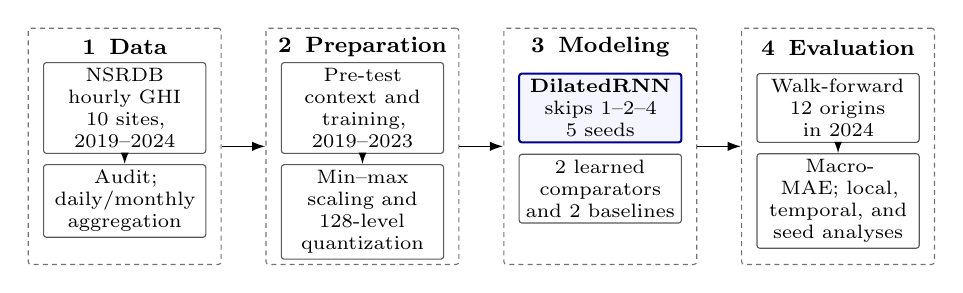
\begin{tikzpicture}[
  stage/.style={
    draw=black!55,
    dash pattern=on 1.8pt off 1.5pt,
    rounded corners=1pt,
    minimum width=2.45cm,
    minimum height=3.00cm,
    inner sep=3pt
  },
  process/.style={
    draw=black!65,
    rounded corners=1pt,
    fill=white,
    align=center,
    text width=1.92cm,
    minimum height=0.68cm,
    inner sep=2pt,
    font=\scriptsize
  },
  proposed/.style={
    process,
    draw=blue!55!black,
    line width=0.75pt,
    fill=blue!4
  },
  stage title/.style={
    font=\footnotesize\bfseries,
    align=center,
    fill=white,
    inner xsep=2pt,
    inner ysep=0pt
  },
  flow/.style={-{Latex[length=1.7mm,width=1.2mm]},line width=0.60pt},
  inner flow/.style={-{Latex[length=1.45mm,width=1.0mm]},line width=0.45pt}
]
  \node[stage] (data-stage) at (0,0) {};
  \node[stage] (prep-stage) at (3.02,0) {};
  \node[stage] (model-stage) at (6.04,0) {};
  \node[stage] (eval-stage) at (9.06,0) {};

  \node[stage title] at ([yshift=-0.25cm]data-stage.north)
    {\textbf{1}\enspace Data};
  \node[process] (raw) at ([yshift=-1.02cm]data-stage.north)
    {NSRDB hourly GHI\\10 sites, 2019--2024};
  \node[process,below=0.13cm of raw] (aggregate)
    {Audit; daily/monthly\\aggregation};

  \node[stage title] at ([yshift=-0.25cm]prep-stage.north)
    {\textbf{2}\enspace Preparation};
  \node[process] (split) at ([yshift=-1.02cm]prep-stage.north)
    {Pre-test context and\\training, 2019--2023};
  \node[process,below=0.13cm of split] (transform)
    {Min--max scaling and\\128-level quantization};

  \node[stage title] at ([yshift=-0.25cm]model-stage.north)
    {\textbf{3}\enspace Modeling};
  \node[proposed] (dilated) at ([yshift=-1.02cm]model-stage.north)
    {\textbf{DilatedRNN}\\skips 1--2--4\\5 seeds};
  \node[process,below=0.13cm of dilated] (comparators)
    {2 learned comparators\\and 2 baselines};

  \node[stage title] at ([yshift=-0.25cm]eval-stage.north)
    {\textbf{4}\enspace Evaluation};
  \node[process] (walk-forward) at ([yshift=-1.02cm]eval-stage.north)
    {Walk-forward\\12 origins in 2024};
  \node[process,below=0.13cm of walk-forward] (metrics)
    {Macro-MAE; local,\\temporal, and seed analyses};

  \draw[inner flow] (raw)--(aggregate);
  \draw[inner flow] (split)--(transform);
  \draw[inner flow] (walk-forward)--(metrics);
  \draw[flow] (data-stage.east)--(prep-stage.west);
  \draw[flow] (prep-stage.east)--(model-stage.west);
  \draw[flow] (model-stage.east)--(eval-stage.west);
\end{tikzpicture}

\caption{End-to-end experimental design. Dashed frames delimit the four stages, and the proposed DilatedRNN is highlighted. Transformations are fitted only on pre-test data; all methods share the 12 test origins in 2024, and learned-model parameters remain fixed during testing.}
\label{fig:pipeline}
\end{figure}

\subsection{Data, Transformations, and Inputs}

The GOES Aggregated Physical Solar Model v4 product of the National Solar Radiation Database (NSRDB) provides satellite-derived, model-based irradiance estimates~\cite{sengupta2018,nlr2026}. Hourly records were averaged first by day and then by calendar month; daily series remained as audited intermediate products. Before modeling, the audit checked dates, metadata, duplicates, gaps, and non-finite or otherwise invalid values. Factory coordinates determined each location's NSRDB grid cell but were not model inputs; a one-hot identifier distinguished sites.

GHI is normalized to $[0,1]$ using minima and maxima estimated exclusively from pre-test data, then clipped to that range and uniformly quantized into 128 levels for every learned model. Inputs comprise the previous 12 monthly GHI values, 3-, 6-, and 12-month moving averages, sine and cosine encodings of the target month, and a one-hot location identifier. The generic one-step forecast is

\begin{equation}
  \widehat y_{\ell,t+1}=f_{\Theta}\!\left(\mathbf{x}_{\ell,t}\right),
  \label{eq:generic}
\end{equation}

where $\ell$ is the location, $t$ the forecast origin, $\mathbf{x}_{\ell,t}$ the available history and covariates, $\widehat y_{\ell,t+1}$ the next-month forecast, and $\Theta$ the learned parameters. MLP uses a tabular representation; DilatedRNN receives the sequence and auxiliary attributes through separate branches; and DeepAR receives the transformed series and location category.

\subsection{Proposed DilatedRNN}

At recurrent layer $k$, the implemented state update uses the state from $s_k$ time steps earlier:

\begin{equation}
  \mathbf h^{(k)}_t=
  \tanh\!\left(
  W^{(k)}_x\mathbf u^{(k)}_t+
  W^{(k)}_h\mathbf h^{(k)}_{t-s_k}+\mathbf b^{(k)}
  \right),\qquad s_k\in\{1,2,4\},
  \label{eq:dilated}
\end{equation}

where $\mathbf u^{(k)}_t$ is the layer input and $\mathbf h^{(k)}_t$ its state; states before the available window are initialized to zero. Each cell maintains a first-in, first-out buffer of $s_k$ states: immediately before processing step $t$, the oldest entry is $\mathbf h^{(k)}_{t-s_k}$; after the update, the buffer advances and receives $\mathbf h^{(k)}_t$. The first two recurrent layers return all 12 states to the next layer, whereas the third returns its final 16-dimensional state. Thus, dilation changes only the recurrent connection and never introduces future observations or treats heterogeneous attributes as artificial time steps.

The auxiliary branch contains the 3-, 6-, and 12-month moving averages, two cyclical target-month encodings, and a ten-component one-hot site identifier. Its 15 values are concatenated with the recurrent representation only after temporal encoding. A dense 16-unit rectified linear unit (ReLU) layer then feeds a scalar linear output. With three 16-unit recurrent layers, this arrangement has 1,873 trainable parameters. Forecasts are transformed back with the pre-test minimum and maximum of the corresponding location and floored at zero to respect the physical lower bound of GHI.

This compact design implements the essential skipped-state transition of Chang et al.~\cite{chang2017} without claiming to reproduce their full architecture. The dilation schedule 1--2--4 provides progressively longer paths within the same annual context, while the 12-month moving average and target-month encoding expose annual structure outside the recurrent state. The fixed context, fixed schedule, simple $\tanh$ cells, and late fusion of auxiliary variables are deliberate controls, but they limit conclusions about other architectures and forecast horizons.

\subsection{Training and Retrospective Evaluation}

The series span 2019--2024. At each location, 2019 provides context for the first target, 48 targets from 2020--2023 form the training period, and the 12 months of 2024 are tested chronologically. Each global learned model thus uses 480 training targets per seed across ten locations.

Data from 2023 selected the number of DilatedRNN epochs. The network was then reinitialized and refitted on all 2020--2023 targets. MLP and DeepAR used configurations fixed before the 2024 evaluation and trained on the complete pre-test period. In walk-forward testing, each newly available monthly value updated the next input context while model parameters remained fixed.

Each learned model was evaluated in five runs with seeds 11, 23, 42, 67, and 89. Point forecasts were averaged across runs, except for DeepAR, whose consolidated forecast was the median of pooled predictive samples. Persistence repeats the preceding month; seasonal naive uses the same month of the previous year. Table~\ref{tab:configuration} reports the verified configurations.

\begin{table}[t]
\caption{Model configurations used in the comparison.}
\label{tab:configuration}
\centering
\scriptsize
\renewcommand{\arraystretch}{1.04}
\begin{tabular}{@{}>{\raggedright\arraybackslash}p{1.75cm}>{\raggedright\arraybackslash}p{9.75cm}@{}}
\toprule
\textbf{Model} & \textbf{Configuration} \\
\midrule
Baselines & Persistence; seasonal naive. \\
MLP & Hidden layers 64--32 with ReLU; L-BFGS; $\alpha=0.05$; at most 2,000 iterations. \\
\textbf{DilatedRNN} & Three 16-unit layers; dilations 1--2--4; context 12; covariates; dense 16-unit ReLU layer; linear output; mean squared error (MSE); Adam 0.001; batch 32; at most 300 epochs; early stopping during selection with patience 30; effective epochs 72, 146, 21, 104, and 69 for seeds 11, 23, 42, 67, and 89. \\
DeepAR & Two 40-unit layers; Student-$t$ output; dropout 0.1; lags 1--12; Adam 0.001; 100 epochs; 50 batches/epoch; batch 32; learning-rate scheduler patience 10. \\
\bottomrule
\end{tabular}
\end{table}

\subsection{Audit, Leakage Control, and Reproducibility}

The audit covered 2,192 daily records per location (21,920 total) from January 1, 2019 through December 31, 2024. It found no invalid dates, non-finite or negative GHI values, duplicates, or missing days. Monthly aggregation followed these checks. Complete daily coverage does not remove uncertainty from the modeled NSRDB reference, but rules out missing-record imputation as an explanation for differences among methods.

All location-wise scales and quantization boundaries were estimated before their test targets became available. Selection on 2023 determined only the DilatedRNN epoch counts; the network was then reinitialized and refitted from scratch. The 120 targets in 2024 were predicted chronologically without weight updates. Retained artifacts include seed-specific predictions, consolidated forecasts, actual hyperparameters, input-file hashes, and the software environment: Python 3.12.1, TensorFlow 2.21.0, PyTorch 2.6.0, and GluonTS 0.16.2. These records support computational auditing, although other hardware and library versions may not reproduce results bit for bit.

\subsection{Metrics}

Let $y_{\ell,i}$ be the NSRDB reference value, $\widehat y_{\ell,i,m}$ the forecast of model $m$, $e_{\ell,i,m}=y_{\ell,i}-\widehat y_{\ell,i,m}$, and $\bar y_\ell$ the mean of the $n_\ell$ test targets. The local metrics are

\begin{equation}
\begin{aligned}
 \mathrm{MAE}_{\ell,m}&=n_\ell^{-1}\sum_i|e_{\ell,i,m}|, &
 \mathrm{MSE}_{\ell,m}&=n_\ell^{-1}\sum_i e_{\ell,i,m}^2,\\
 \mathrm{RMSE}_{\ell,m}&=\sqrt{\mathrm{MSE}_{\ell,m}}, &
 R^2_{\ell,m}&=1-\frac{\sum_i e_{\ell,i,m}^2}{\sum_i(y_{\ell,i}-\bar y_\ell)^2},\\
 \mathrm{nRMSE}_{\ell,m}(\%)&=100\,\mathrm{RMSE}_{\ell,m}/\bar y_\ell. &&
\end{aligned}
\label{eq:metrics}
\end{equation}

The primary criterion is macro-MAE, the unweighted mean of ten local MAEs~\cite{hyndman2006}. MSE and RMSE emphasize large errors, $R^2$ measures tracked variation, and nRMSE expresses RMSE relative to mean GHI. Metrics are averaged after local calculation; thus, mean RMSE is not the square root of mean MSE. The standard-deviation column in Table~\ref{tab:overall} gives the sample standard deviation of macro-MAE across seeds.

\section{Results and Discussion}
\label{sec:results}

\subsection{Overall Model Comparison}

Table~\ref{tab:overall} is ordered by macro-MAE. Among the five methods compared, DilatedRNN ranked first by macro-MAE; it also ranked first among the three learned models. Its MAE of 13.42~W/m$^2$ was 0.76~W/m$^2$ (5.36\%) lower than the 14.18~W/m$^2$ obtained by the second-ranked model, DeepAR.

\begin{table}[t]
\caption{Mean metrics across the ten locations in the retrospective test.}
\label{tab:overall}
\centering
\scriptsize
\setlength{\tabcolsep}{3.2pt}
\begin{tabular}{@{}lrrrrrr@{}}
\toprule
\textbf{Model} & \textbf{MAE} & \textbf{SD} & \textbf{MSE} & \textbf{RMSE} & \textbf{$R^2$} & \textbf{nRMSE} \\
 & \textbf{W/m$^2$} & \textbf{W/m$^2$} & \textbf{W$^2$/m$^4$} & \textbf{W/m$^2$} & & \textbf{\%} \\
\midrule
\textbf{DilatedRNN} & \textbf{13.42} & \textbf{0.83} & \textbf{286.63} & \textbf{16.20} & \textbf{0.898} & \textbf{7.93} \\
DeepAR         & 14.18 & 0.90 & 336.88  & 17.94 & 0.892 & 8.78 \\
MLP            & 16.06 & 0.46 & 418.44  & 19.77 & 0.875 & 9.70 \\
Seasonal naive & 16.94 & --   & 496.86  & 21.37 & 0.829 & 10.38 \\
Persistence    & 35.09 & --   & 1808.74 & 42.17 & 0.576 & 20.89 \\
\bottomrule
\end{tabular}
\end{table}

Relative to the two simple baselines, DilatedRNN reduced MAE by 20.78\% against seasonal naive and by 61.75\% against persistence. Its seed-to-seed standard deviation of 0.83~W/m$^2$ was the second largest among learned models, below only DeepAR's 0.90~W/m$^2$, indicating moderate initialization sensitivity. Its lowest RMSE and nRMSE, together with its highest $R^2$, show that the aggregate advantage was not restricted to the primary metric.

\subsection{DilatedRNN Performance by Location}

Table~\ref{tab:local} uses the mean forecast across the five seeds. Its SD column is the sample standard deviation of the five local MAEs, not a probabilistic prediction interval.

\begin{table}[t]
\caption{DilatedRNN performance by location.}
\label{tab:local}
\centering
\scriptsize
\setlength{\tabcolsep}{2.7pt}
\begin{tabular}{@{}>{\raggedright\arraybackslash}p{3.05cm}rrrrrr@{}}
\toprule
\textbf{Location} & \textbf{MAE} & \textbf{SD} & \textbf{MSE} & \textbf{RMSE} & \textbf{$R^2$} & \textbf{nRMSE} \\
 & \textbf{W/m$^2$} & \textbf{W/m$^2$} & \textbf{W$^2$/m$^4$} & \textbf{W/m$^2$} & & \textbf{\%} \\
\midrule
BMW San Luis Potosí & 20.92 & 3.44 & 621.48 & 24.93 & 0.692 & 10.06 \\
BYD Camaçari        & 16.83 & 2.47 & 495.90 & 22.27 & 0.646 & 9.43 \\
Ford Rouge          & 12.67 & 1.64 & 210.28 & 14.50 & 0.965 & 9.04 \\
GM Factory Zero     & 12.38 & 0.94 & 206.05 & 14.35 & 0.965 & 8.96 \\
Hyundai Georgia     & 12.96 & 1.13 & 257.23 & 16.04 & 0.914 & 8.09 \\
Lucid Casa Grande   & 8.40  & 0.66 & 118.70 & 10.90 & 0.979 & 4.42 \\
Rivian Normal       & 18.45 & 1.81 & 459.08 & 21.43 & 0.922 & 11.91 \\
Tesla Fremont       & 7.45  & 2.59 & 83.40  & 9.13  & 0.991 & 4.14 \\
Tesla Nevada        & 10.49 & 2.00 & 143.89 & 12.00 & 0.984 & 5.40 \\
Tesla Texas         & 13.67 & 2.07 & 270.32 & 16.44 & 0.919 & 7.87 \\
\bottomrule
\end{tabular}
\end{table}

Local MAE ranged from 7.45~W/m$^2$ at Tesla Fremont to 20.92~W/m$^2$ at BMW San Luis Potosí, a spread of 13.47~W/m$^2$. DilatedRNN ranked first at GM Factory Zero, Rivian, Tesla Fremont, and Tesla Nevada; second at BMW, Ford, Lucid, and Tesla Texas; and third at BYD and Hyundai. It outperformed seasonal naive at eight locations and persistence at all ten; seasonal naive was better at Ford and Lucid. RMSE ranged from 9.13~W/m$^2$ at Fremont to 24.93~W/m$^2$ at BMW; seed-to-seed SD ranged from 0.66~W/m$^2$ at Lucid to 3.44~W/m$^2$ at BMW. These differences show both regional heterogeneity and location-dependent initialization sensitivity.

Against DeepAR specifically, DilatedRNN obtained lower local MAE at six of ten sites. Its largest relative advantages occurred at Tesla Fremont (39.81\%) and Tesla Nevada (33.81\%), whereas its largest deficit occurred at Tesla Texas (36.18\%). The median relative advantage over DeepAR across locations was 3.30\%. Thus, the 5.36\% aggregate gain did not arise from uniform improvements and should not be interpreted as a site-independent effect.

\subsection{Seed Variability and Example Forecast}

Across five runs, macro-MAE ranged from 13.22~W/m$^2$ (seed 23) to 15.18~W/m$^2$ (seed 42), a spread of 1.96~W/m$^2$. The consolidated mean forecast attained 13.42~W/m$^2$: it outperformed the forecasts from four individual runs but did not outperform the best run. This distinction matters because the reported consolidated metric measures an ensemble forecast, while the SD in Table~\ref{tab:overall} describes training variability across runs.

\begin{figure}[t]
\centering
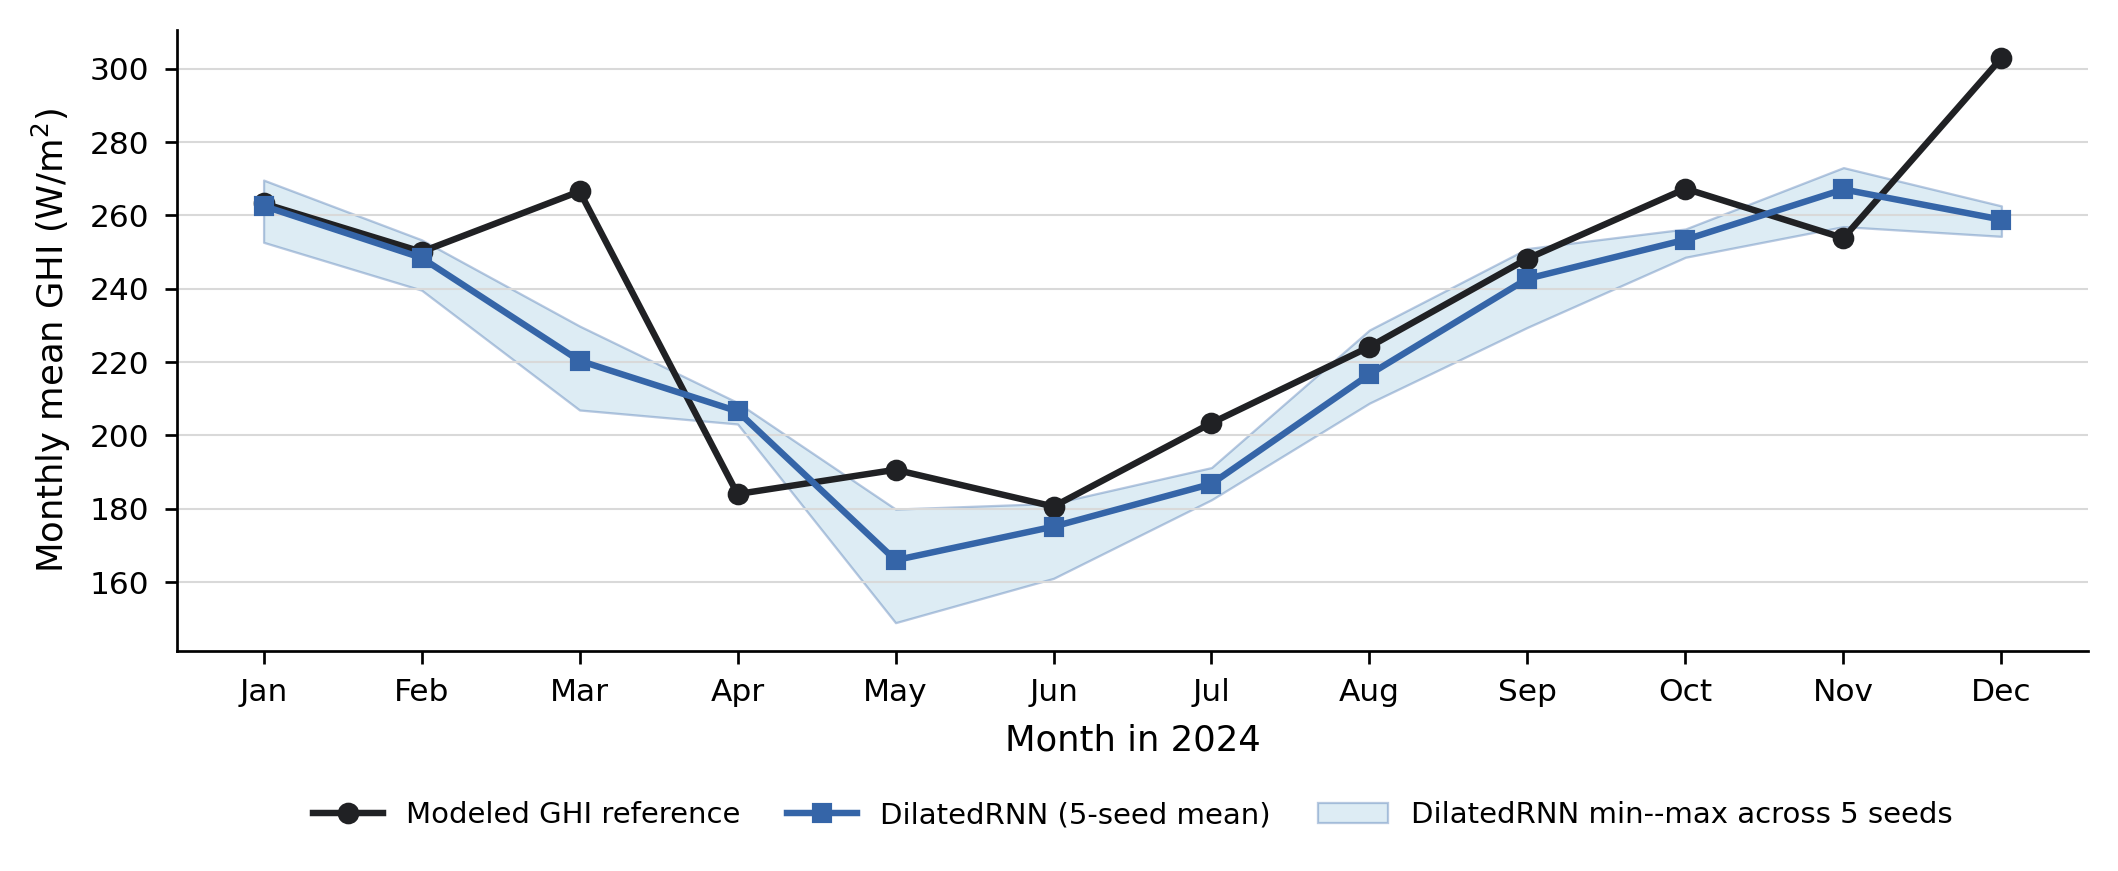
\includegraphics[width=0.90\textwidth]{dilatedrnn_forecast_byd_camacari.png}
\caption{Monthly GHI forecasts for BYD Camaçari in 2024. The DilatedRNN band shows the range of forecasts across five random seeds and is not a calibrated probabilistic interval.}
\label{fig:camacari}
\end{figure}

Figure~\ref{fig:camacari} illustrates Camaçari, a challenging case in which DilatedRNN ranked third. The smallest absolute errors occurred in January (0.69~W/m$^2$) and February (1.64~W/m$^2$). The network followed the decline from March to June and the subsequent seasonal increase, but it smoothed the March and December peaks, producing its largest errors of 46.17 and 44.03~W/m$^2$, respectively. Its annual MAE was 16.83~W/m$^2$. The monthly standard deviation across seeds averaged 6.33~W/m$^2$ and reached 11.22~W/m$^2$ in May. Five runs do not define a calibrated predictive distribution.

\subsection{Paired Descriptive Error Comparison}

Aggregate MAE does not show how consistently one method wins at individual forecast origins. Table~\ref{tab:paired} therefore compares absolute errors pairwise at the same 120 location--month targets. A win for DilatedRNN denotes a strictly smaller absolute error than the comparator's; there were no ties. The mean gap is the comparator's absolute error minus that of DilatedRNN, so positive values favor the proposed model. These are descriptive matched counts, not independent trials.

\begin{table}[H]
\caption{Paired absolute-error comparison over the 120 test targets.}
\label{tab:paired}
\centering
\scriptsize
\setlength{\tabcolsep}{5.0pt}
\begin{tabular}{@{}lrrrr@{}}
\toprule
\textbf{Comparator} & \textbf{Wins} & \textbf{Losses} & \textbf{Win rate} & \textbf{Mean gap (W/m$^2$)} \\
\midrule
DeepAR         & 66 & 54 & 55.0\% & 0.76 \\
MLP            & 75 & 45 & 62.5\% & 2.64 \\
Seasonal naive & 63 & 57 & 52.5\% & 3.52 \\
Persistence    & 97 & 23 & 80.8\% & 21.67 \\
\bottomrule
\end{tabular}
\end{table}

DilatedRNN recorded more wins than losses against DeepAR, MLP, and both baselines. A post hoc analysis of upper-tail errors further showed that its absolute error exceeded 30~W/m$^2$ for 8 of the 120 targets, compared with 14 for DeepAR, 15 for MLP, 23 for seasonal naive, and 58 for persistence. These matched results strengthen the error-profile interpretation, but they do not estimate future win probabilities because the targets cover a single year and are temporally and spatially dependent.

\subsection{Limitations}

Only four annual cycles were available for training, five runs with different random seeds were evaluated, and the single retrospective test window also informed development decisions. The 120 monthly test targets are not a random sample: months within a location are serially related, and nearby sites may share regional conditions. Consequently, no hypothesis test treating all target errors as independent is reported.

The NSRDB reference consisted of model-based estimates rather than measurements collected at the factories, and the raw hourly records were not preserved. The factory-associated locations constitute a convenience sample. Clipping and quantization were applied to all learned models but not to the two baselines. The 12-month context and dilation factors were fixed, no future meteorological covariates were supplied, and the comparison did not constitute an exhaustive search over architectures or hyperparameters. No industrial data were involved. Generalization to other periods, regions, ground measurements, photovoltaic generation, and forecast horizons therefore requires a new prospective evaluation.

\section{Conclusion}
\label{sec:conclusion}

The proposed global model achieved a location-averaged MAE of 13.42~W/m$^2$ and a seed-to-seed SD of 0.83~W/m$^2$ across ten locations. Among the five methods compared, DilatedRNN ranked first by macro-MAE but led at only four locations; local MAE ranged from 7.45 to 20.92~W/m$^2$.

The 1--2--4 recurrent skips represented distinct temporal scales without preventing peak smoothing or regional sensitivity. The model's more favorable upper-tail error profile supported the aggregate result, although performance still varied by location. With four training cycles and one retrospective window, the evidence supports competitive, not universally superior, performance. Future work should extend the historical record, test other context lengths and dilation schedules, include meteorological covariates, and reserve new periods for prospective evaluation.

\begin{credits}
\subsubsection{Acknowledgments.}
The authors acknowledge financial support from FAPEMIG (grant OET-00243-26).

\subsubsection{Disclosure of Interests.}
The authors have no competing interests to declare that are relevant to the content of this article.
\end{credits}

\begin{thebibliography}{10}

\bibitem{chang2017}
Chang, S., Zhang, Y., Han, W., Yu, M., Guo, X., Tan, W., Cui, X., Witbrock, M., Hasegawa-Johnson, M.A., Huang, T.S.:
Dilated recurrent neural networks. In: Advances in Neural Information Processing Systems, vol.~30 (2017)

\bibitem{hewamalage2021}
Hewamalage, H., Bergmeir, C., Bandara, K.:
Recurrent neural networks for time series forecasting: Current status and future directions. International Journal of Forecasting \textbf{37}(1), 388--427 (2021). \doi{10.1016/j.ijforecast.2020.06.008}

\bibitem{hyndman2006}
Hyndman, R.J., Koehler, A.B.:
Another look at measures of forecast accuracy. International Journal of Forecasting \textbf{22}(4), 679--688 (2006). \doi{10.1016/j.ijforecast.2006.03.001}

\bibitem{jung2020}
Jung, Y., Jung, J., Kim, B., Han, S.:
Long short-term memory recurrent neural network for modeling temporal patterns in long-term power forecasting for solar PV facilities: Case study of South Korea. Journal of Cleaner Production \textbf{250}, 119476 (2020). \doi{10.1016/j.jclepro.2019.119476}

\bibitem{montero2021}
Montero-Manso, P., Hyndman, R.J.:
Principles and algorithms for forecasting groups of time series: Locality and globality. International Journal of Forecasting \textbf{37}(4), 1632--1653 (2021). \doi{10.1016/j.ijforecast.2021.03.004}

\bibitem{nlr2026}
National Laboratory of the Rockies:
National Solar Radiation Database API documentation. \url{https://developer.nlr.gov/docs/solar/nsrdb/}, last accessed 2026/08/03

\bibitem{ozoegwu2019}
Ozoegwu, C.G.:
Artificial neural network forecast of monthly mean daily global solar radiation of selected locations based on time series and month number. Journal of Cleaner Production \textbf{216}, 1--13 (2019). \doi{10.1016/j.jclepro.2019.01.096}

\bibitem{salinas2020}
Salinas, D., Flunkert, V., Gasthaus, J., Januschowski, T.:
DeepAR: Probabilistic forecasting with autoregressive recurrent networks. International Journal of Forecasting \textbf{36}(3), 1181--1191 (2020). \doi{10.1016/j.ijforecast.2019.07.001}

\bibitem{sengupta2018}
Sengupta, M., Xie, Y., Lopez, A., Habte, A., Maclaurin, G., Shelby, J.:
The National Solar Radiation Data Base (NSRDB). Renewable and Sustainable Energy Reviews \textbf{89}, 51--60 (2018). \doi{10.1016/j.rser.2018.03.003}

\bibitem{voyant2017}
Voyant, C., Notton, G., Kalogirou, S., Nivet, M.-L., Paoli, C., Motte, F., Fouilloy, A.:
Machine learning methods for solar radiation forecasting: A review. Renewable Energy \textbf{105}, 569--582 (2017). \doi{10.1016/j.renene.2016.12.095}

\bibitem{voyant2022}
Voyant, C., Notton, G., Fouilloy, A., Duchaud, J.-L., Nivet, M.-L.:
Benchmarks for solar radiation time series forecasting. Renewable Energy \textbf{191}, 747--762 (2022). \doi{10.1016/j.renene.2022.04.065}

\end{thebibliography}

\end{document}
